\chapter{\centering Software Description}

\section{GUI}
% Developed by using java Swing but since default does not look appealing, we decided to download a dependency called Flat LaF (look and feel) to change the theme of our overall application making it look more up to date with current application standards.

Initially developed using default java swing, we have decided to use a dependency called \emph{FlatLaf} that allows our application to have aesthetics that is up to date with other current applications' standards, since the look of the default swing framework is rather outdated.

\section{User Registration}

\subsection{Login Page}
The login page is the first page that the user will encounter when they start the app. The page is 
capable of displaying error messages such as: empty email or password field, incorrect email format by using the regex
function to check, and finally display an error message indicating whether the information entered is correct or valid for the user to be
logged in.

\begin{figure}[ht]
	\centering
	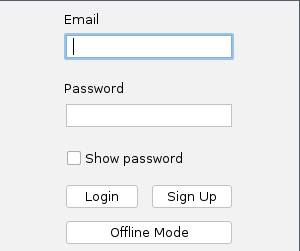
\includegraphics[scale=0.5,keepaspectratio]{Figures/login_page.png}
    \caption{Login page image}
    \label{fig:loginPage}
\end{figure}

Two accounts exist on the remote database that are used purely for testing:
\begin{itemize}
    \item Normal user account email: t@g.com, password: t
    \item Admin user account email: f@g.com, password: f
\end{itemize}

The login page can automatically detect whether the user is an admin or a normal user and redirect them to the corresponding
page.

\subsection{Sign Up Page}
\label{subsection:signup}
If the user is a first time user and doesn't have an account, they can click on the sign up button to be redirected to the sign up page,after which they will be able to create an account by entering an email, password and username. Email and password are required to log into the app and the username will be used to display to other user and in the setting page,this is done because though the email is unique, the username is not, along our user to have a professional and recognizable name to refer to each others. 

If users click on the sign up page by mistake, there is an "already have an account?" button where they can be redirected back to the 
login page.  

An admin account can not be created from the sign up page. But a normal user can be elevate to admin status by an existing admin
using the edit button that they have in their admin page.

\begin{figure}[ht]
	\centering
	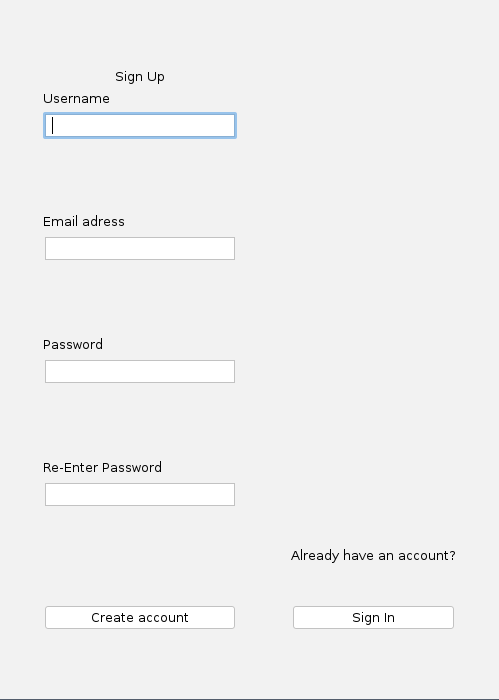
\includegraphics[scale=0.5,keepaspectratio]{Figures/sign_up.png}
	 \caption{Admin page image}
     \label{fig:adminPage}
\end{figure}

\section{Event Page}
Main page of our time scheduler. Here the user has access to most functions of the software.
\subsection{Calendar View}
A live calendar is displayed using the current time of the user's computer as the initial month. Each cell represents a day of the month and can be clicked to open a new frame, showing all events of that day. The cells are highlighted by colours if an event is in our database on that day. The colour changes based on priority from green to red. By clicking the << or >> buttons at the top, the user can change the displayed month of the calendar
\subsection{Side Bar}
Includes a button labeled as "New Event" to access the Add Event page where you can create a new event. The Upcoming Events panel shows you a list of your current events. Lastly the Sync button allows the user to synchronize with the remote database.
\subsection{Adding Events}
A frame allowing to the user to add new events to his scheduler. It can be opened either by using the add event button on the main page or by clicking the add button on the show events page. The user input is checked to avoid invalid inputs.
\subsection{Show Events}
A frame showing all events of single day. It can be opened by clicking on a cell in our calendar. When
an event from the list is clicked, a new frame called Edit Event with additional information about that event is created.
\subsection{Edit Events}
A frame allowing the user to edit information about an event or delete it. It is almost identical in design to the Add Event frame.
\section{Database}
Our application currently operates on two SQL database.
\subsection{Remote}
Database server hosted by Frankfurt UAS faculty 2 for the course Database taught by Prof. Dr. Christian Rich. Connect to the
database using Triet Huynh account assigned to him in the previously mentioned course as learning resource. The database
is using Oracle SQL\texttrademark  and is run constantly 24/7. This is the database that the user interacting with when login,
sign up or use any of the functionalities in the admin page. 

\subsection{Local}
The database is run locally on the user's computer using SQLite version 3036000. SQLite is a light weight implementation of a
DBMS, allowing us to store and retrieve data that doesn't require the user to install anything to be able to interact with the local database. Connection to the local database has almost no latency and is reliable. 
Connection to the local database is only established after the user has finished login or sign up, connection is then terminated when user closed the app.

\section{Security}
\subsection{Password Encryption}
To protect the user from the aftermath of a security breach of our remote server.The user's password is hashed using
sha2-256 locally on the user computer via the application. The remote database only stores the hashed password.

% \subsection{Error message display on incorrect login}
% We decided to show the same error message "Email or password incorrect" in case of the email entered in the login field 
% either does not exist on the remote database and/or is a typo, as well as
% the password entered is incorrect for that account. This is done since an error message i.e. "Account
% with this email address does not exist" would have been displayed at a login try and that will indicate to the malicious hacker or other people that want to 
% gain access to the account the knowledge that the email they have just entered is correct and they now only need to find the correct
% password.

% \subsection{Login page error message}
% The login page will show the same error message both cases if either the user does with that email does not
% exist or the password is entered incorrectly. This is done to provide less information to unauthorized
% people that want to gain access to an account.

% To authenticate the user when they are logging in, the hashed password is then download from the remote database. Then the 
% user entered password from the password field is hashed with the same hash algorithm, the two String is then compare against
% each other.

\section{Admin Page}
The administrator (admin) has extended rights, an individual GUI with a full view/access to the user profiles in the database and executes commands like changing a username or email and the possibility to completely delete a user from the database.  
Admins do not have access to event pages. The admin sole purpose is user database administration.
\subsection{Edit}
The admin has the option to edit the username and/or email of a user if it's i.e. not appropriate and the admin feels that it has to be changed or the user wishes for a name change. The changes will be saved in the database and updated on every other part of the app where the email/username has to be displayed.

\subsection{Delete}
The admin also has the capability to delete a user in case he wants his account deleted for personal reasons or if he has an impression of the user violating the terms of service (i.e. misbehavior, profanity). In case this happens, the user will then be fully deleted and non-existent in the database or application.

\section{Email Function}
The emailUtils class contains all the necessary tools to establish a connection to the gmail servers and a method that is used i.e. to send out predefined automated reminders (depending on the reminder selected) or notifications when events are changed/deleted via user emails passed in as parameters to the participants. It has the option to modify the header/subject and the body (main message) of the email (passed in as parameters as well).

\section{Menu Bar}
The Menu Bar has several drop down menus like Export, About, and most importantly the Menu. There we have the access for the user to the Profile Page, Settings, as well as a Log Out and Exit options.
\subsection{Profile}
The Profile page welcomes the user and displays the superficial details as in username and email but also gives the ID number for each user. Additionally the Profile page shows a Contacts section where the user may enter the Contacts page.
\subsection{Settings}
If the User want change any part of their details, they can make those changes themselves by using the Settings page which offers three methods to change each attribute of the current user.
\subsection{Contacts}
The User has a contact list. This page allows you the options to Add and Delete contacts from your personal contact list. They will then  appear in the add "Participant" tab in the event creation for a day.

\subsection{Database}
% Includes buttons to handle the local database
Include two buttons to export and import the local database.

% \subsubsection{Export Database}
% export the database file to a .db file on the user's computer.

% \subsubsection{Import Database}
% import a SQLite file on the user's computer to be used. The application must be restart for the 
% changes to take effect